\chapter{User Interface}
\label{chapter_ui}

This chapter, as apparent from its name, is considered as a reference card for the MITHRA code.
%
We aim to present the functions and variables which can be delivered to the MITHRA software and can be handled for a FEL simulation problem.
%
In what follows in this chapter, we introduce the defined language of MITHRA to write a compatible job file.
%
This chapter can also be considered as a reference for the current capabilities of MITHRA and with time will be updated with the further improvement of the software capabilities.
%
\begin{description}
\item[\textbf{Iron Rule:}] parameters that are used for the solution of a specific electromagnetic problem are delivered to the code at only one single location, \emph{the job file}. This is indeed the only thing that the solver takes as an input parameter.
\end{description}
%
It should be noted that all the parameters in the job file is given in the laboratory frame.
%
The Lorentz boost into the bunch rest frame will be done by the software automatically.

To run a job file using the software MITHRA, the following command should be written in the linux command line:

\begin{itemize}
	\item  mpirun -np "number of distributed processors" "MITHRA object file name" "job file name"
\end{itemize}

The transferred job file to the solver contains five main sections, each one defining an essential part of the electromagnetic problem.
%
These sections include:
%
\begin{enumerate}
\item \textbf{\texttt{MESH:}} The parameters of the FDTD solver like the computational domain, cell sizes and time steps are set in this section.
\item \textbf{\texttt{BUNCH:}} The required data to initialize the electron bunch in the computational domain is set in this section. In addition, the desired type of recording the bunch evolution is entered in this section by the user.
\item \textbf{\texttt{FIELD:}} This section fulfills the same task as the previous section for the electromagnetic fields. The field initialization in case of a seeded FEL and the desired output type for the field evolution is given in this section to the software.
\item \textbf{\texttt{UNDULATOR:}} This section introduced the different parameters of the undulator.
\item \textbf{\texttt{EXTERNAL-FIELD:}} This section introduces the fields of some external components to the FEL interaction. It is relatively rare to have external components superimposed on the undulator field. However, such a possibility enables studying novel and advanced FEL cases.
\item \textbf{\texttt{FEL-OUTPUT:}} The desired data concerning the FEL radiation and how to record this data is set in this section.
\end{enumerate}
%
In the next subsections, we explain each part and the supported parameters, respectively.
%
To write comments in your job file use the sign "\#" at the beginning of the comment and the text will be commented to the end of the line.

\section{\texttt{MESH}}

As mentioned above, this part is dedicated to the determination of the FDTD/PIC parameters.
%
In Fig\,\ref{RefcardFig1}, a typical computation domain assumed in MITHRA is depicted.
%
\begin{figure}
\centering
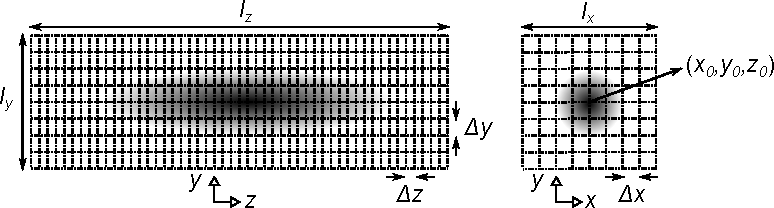
\includegraphics[width=5.0in]{./MITHRA_UI/Fig1.pdf}
\caption{The definition of the spatial mesh parameters in MITHRA}
\label{RefcardFig1}
\end{figure}
%
The mesh and update parameters of the solver are defined through the following eleven parameters:
%
\begin{itemize}
\item \textbf{\texttt{length-scale}} is the scaling of the length and all the spatial parameters in the job file. The capability to play with length scales is crucial to avoid working with very large or very small numbers.
\item \textbf{\texttt{time-scale}} is the scaling of the time and all the temporal parameters in the job file. Similar to above, through this capability working with very large or very small numbers is avoided.
\item \textbf{\texttt{mesh-lengths}} is a three dimensional vector equal to the lengths $(l_x,l_y,l_z)$ of the computational domain (\ref{RefcardFig1}) along the three Cartesian axes.
\item \textbf{\texttt{mesh-resolution}} defines the length of one single grid cell or in other words the spatial discretization resolution of the FDTD mesh in the laboratory coordinate system $(\Delta x',\Delta y',\Delta z')$.
\item \textbf{\texttt{mesh-center}} is the position of the central point of the computational rectangle, i.e. $(x_0',y_0',z_0')$ in Fig.\,\ref{RefcardFig1}.
\item \textbf{\texttt{total-time}} is the total computation time in the scale given by the time scale. This is indeed the time it takes for the electron bunch to travel through the considered undulator length.
\item \textbf{\texttt{bunch-time-step}} is the time step for updating the macro-particles' coordinates in the PIC solver.
\item \textbf{\texttt{bunch-time-start}} is the time point when the bunch of macro-particles emerges in the computational domain.
\item \textbf{\texttt{mesh-truncation-order}} is the truncation order of the absorbing boundary condition in the computational domain. This parameter can be either 1 or 2, representing the first order and second order absorbing boundary condition.
\item \textbf{\texttt{space-charge}} is a boolean flag determining if the space-charge effect should be considered or not. If this flag is false, the scalar potential $\phi$ is zero throughout the calculation. Otherwise, the scalar potential is calculated using the corresponding Helmholtz equation.
\end{itemize}

The format of the \texttt{MESH} group is:
%%
\begin{Verbatim}[frame=single,fontsize=\small,tabsize=4]
MESH
{
	length-scale                    = < real value | METER | DECIMETER | CENTIMETER | MILLIMETER
									  | MICROMETER | NANOMETER | ANGSTROM >
	time-scale                      = < real value | SECOND | MILLISECOND | MICROSECOND |
									  NANOSECOND | PICOSECOND | FEMTOSECOND | ATTOSECOND >
	mesh-lengths                    = < ( real value,  real value, real value) >
	mesh-resolution                 = < ( real value,  real value, real value) >
	mesh-center                     = < ( real value,  real value, real value) >
	total-time                      = < real value >
	bunch-time-step                 = < real value >
	bunch-time-start                = < real value >
	mesh-truncation-order           = < 1 | 2 >
    space-charge           	     = < true | false >
}
\end{Verbatim}
%%
An example of the computational mesh definition looks as the following:
%%
\begin{snugshade}
\begin{Verbatim}[fontsize=\small, tabsize = 4]
MESH
{
  length-scale                      = MICROMETER
  time-scale                        = PICOSECOND
  mesh-lengths                      = ( 3200,  3200.0,    280.0)
  mesh-resolution                   = ( 50.0,    50.0,      0.1)
  mesh-center                       = ( 0.0,      0.0,      0.0)
  total-time                        = 30000
  bunch-time-step                   = 1.6
  bunch-time-start                  = 0.0
  mesh-truncation-order             = 2
  space-charge                      = false
}
\end{Verbatim}
\end{snugshade}
%
Note that there are some conditions, which should be fulfilled for the numerical integrator to obtain reliable dispersion-less results.
%
The software checks for these conditions before starting to solve the problem, if the conditions are violated the closest value to the given number meeting the violated conditions will be used.
%
Regarding the above parameters. the software checks for the stability condition $\sqrt{(\Delta z/\Delta x)^2+ (\Delta z/\Delta y)^2} < 1$, adapts the values of $\Delta x$ and $\Delta y$ accordingly, and finally sets the time step for field update equal to $\Delta z / c$.
%
In addition, the bunch update time step should be an integer fraction of the field time step to avoid redundant dispersion in the calculated values.
%
Therefore, the closest value to the given bunch time step, which satisfies the above criterion, will be chosen.

\section{\texttt{BUNCH}}

The section \texttt{BUNCH} is the main part of the job file to establish the required data for the bunch input and output framework.
%
This section consists of four groups: (1) \texttt{bunch-initialization}, (2) \texttt{bunch-sampling}, (3) \texttt{bunch-visualization}, and (4) \texttt{bunch-profile}.
%
As apparent from the name the first group determines the set of parameters to initialize the bunch and the other three groups are dedicated to reporting the bunch evolution in different formats.
%
In what follows, the parameters in each group are introduced:

\begin{enumerate}
\item \textbf{\texttt{bunch-initialization:}} This group mainly determines the parameters whose values are needed for initializing a bunch of electrons with different types. If several bunches are present in a simulation, this group should simply be repeated in the \texttt{BUNCH} section. The set of values accepted in this group include:
\begin{itemize}
\item \textbf{\texttt{type}} is the type of the bunch to be initialized in the computational domain. There are five bunch types supported by MITHRA:
\begin{enumerate}
	\item \texttt{manual} initializes charges at the points specified by the position vector. At each appearance of this type of bunch only one single macro-particle will be initialized. Therefore, to have multiple manual initialization, the \texttt{bunch-initialization} group should be repeated. Using the \texttt{file} type is a better solution for high number of manual inputs.
	\item \texttt{ellipsoid} initializes charges with a
	\item \texttt{3D-crystal} initializes multiple bunches on the points of a 3D crystal centered at the coordinate specified by the position vector and extends over the space by the number vector and the considered lattice constant. Each single bunch has a ellipsoid Gaussian property with the values read from the deviation parameters.
	\item \texttt{file} reads a list of 6D position and momentum coordinates from a file and initializes the macro-particles correspondingly in the solver.
\end{enumerate}
\item \textbf{\texttt{distribution}} determines if the initialized particle distribution should have a uniform or Gaussian current profile.
\item \textbf{\texttt{number-of-particles}} is the total number of particles (or macro-particles) considered in the bunch.
\item \textbf{\texttt{charge}} is the total charge of the bunch in one electron charge unit.
\item \textbf{\texttt{gamma}} is the initial mean Lorentz factor of the .
\item \textbf{\texttt{beta}} is the initial mean normalized velocity of the particles, if it is not determined here the value will be calculated from the \texttt{gamma} parameter, otherwise the same \texttt{beta} will be used.
\item \textbf{\texttt{direction}} is the average momentum direction of the bunch, i.e. $(\beta_x, \beta_y, \beta_z)/\beta$.
\item \textbf{\texttt{position}} is the central position of the bunch.
\item \textbf{\texttt{sigma-position}} is the deviation in position of the bunch, i.e. $(\sigma_x, \sigma_y, \sigma_z)$ for Gaussian distributions. $\sigma_z$ half the bunch length for the uniform distribution.
\item \textbf{\texttt{sigma-momentum}} is the deviation in energy of the bunch, i.e. $(\sigma_{\gamma \beta_x}, \sigma_{\gamma \beta_y}, \sigma_{\gamma \beta_z})$.
\item \textbf{\texttt{numbers}} is a parameter read only when the bunch type is a \texttt{3d-crystal} type. It is the number of bunch replication in the three directions.
\item \textbf{\texttt{lattice-constants}} is a parameter read only when the bunch type is a \texttt{3d-crystal} type. It is the length of lattice constants of the crystal in the three directions.
\item \textbf{\texttt{transverse-truncation}} determines a limit to transversely truncate the bunches. This factor brings the possibility to control particle initialization and prevents them from escaping out of the computational domain. The bunch initializer truncates the bunch at the given distance from the bunch center.
\item \textbf{\texttt{longitudinal-truncation}} determines a limit to longitudinally truncate the bunches. This factor brings the possibility to control particle initialization and prevents them from escaping out of the computational domain. The bunch initializer truncates the bunch at the given distance from the bunch center.
\item \textbf{\texttt{bunching-factor}} is a value larger than zero and less than one, which determines the bunching factor, i.e. $<e^{jk_uz}>$, of the initialized bunch.
\end{itemize}
%%
\item \textbf{\texttt{bunch-sampling:}} This group defines the required parameters for saving the bunch properties with time. The bunch mean position, mean momentum, position spread, and momentum spread along the three Cartesian coordinates are saved respectively with time. There are different parameters required for this definition which include:
\begin{itemize}
	\item \textbf{\texttt{sample}} is a boolean value determining if the bunch sampling should be activated.
	\item \textbf{\texttt{base-name}} is the file name (no suffix) with the required address of the file to save the output data.
	\item \textbf{\texttt{directory}} is the address where the above file should be saved. The file name with the address can also be given in the base-name section. The software eventually considers the combination of directory and base-name as the final complete file name.
	\item \textbf{\texttt{rhythm}} is the rhythm of bunch sampling, i.e. the time interval between two consecutive visualization times.
\end{itemize}
%%
\item \textbf{\texttt{bunch-visualization:}} This group defines the required parameters for visualizing the charge distribution in the whole computational domain. The output will be a set of \texttt{.vtu} files at each time for each processor which are connected with a set of \texttt{.pvtu} files. They can be very nicely visualized using the open source ParaView package. There are different parameters required for this definition which include:
\begin{itemize}
	\item \textbf{\texttt{sample}} is a boolean value determining if the charge visualization should be activated.
	\item \textbf{\texttt{base-name}} is the file name (no suffix) with the required address of the file to save the output data.
	\item \textbf{\texttt{directory}} is the address where the above file should be saved. The file name with the address can also be given in the base-name section. The software eventually considers the combination of directory and base-name as the final complete file name.
	\item \textbf{\texttt{rhythm}} is the rhythm of charge illustration, i.e. the time interval between two consecutive visualization times.
\end{itemize}
%%
\item \textbf{\texttt{bunch-profile:}} This group defines the required parameters for saving a histogram of the charges. It means that at a specific time instant the charge values, positions and momenta of all the particles (or macro-particles) will be written and saved in a file. The parameters entered by the user for saving the histogram include:
\begin{itemize}
	\item \textbf{\texttt{sample}} is a boolean value determining if the writing of the histogram during the PIC simulations should be activated.
	\item \textbf{\texttt{base-name}} is the file name (no suffix) with the required address of the file to save the output data.
	\item \textbf{\texttt{directory}} is the address where the above file should be saved. The file name with the address can also be given in the base-name section. The software eventually considers the combination of directory and base-name as the final complete file name.
	\item \textbf{\texttt{time}} is the time instant for saving the histogram. If this needs to be done in several time instants, simply this line should be repeated with different time values.
    \item \textbf{\texttt{rhythm}} is the rhythm of writing the bunch profile, i.e. the time interval between two consecutive profiling times. If this value is nonzero, the sequence of times will be considered in addition to the specific time points given by the time variable.
\end{itemize}
\end{enumerate}

The format of the \texttt{BUNCH} group is:
%%
\begin{Verbatim}[frame=single,fontsize=\small,tabsize=4]
BUNCH
{
	bunch-initialization
	{
		type                        = < manual | ellipsoid | 3D-crystal | file >
		distribution                = < uniform | gaussian >
		charge                      = < real value >
		number-of-particles         = < integer value >
		gamma                       = < real value >
		beta                        = < real value >
		direction                   = < ( real value, real value, real value ) >
		position                    = < ( real value, real value, real value ) >
		sigma-position              = < ( real value, real value, real value ) >
		sigma-momentum              = < ( real value, real value, real value ) >
		transverse-truncation       = < real value >
		longitudinal-truncation     = < real value >
		bunching-factor             = < real value between zero and one >
	}
	
	bunch-sampling
	{
		sample                      = < true | false >
		directory                   = < address according to UNIX convention >
		base-name                   = < name of the file >
		rhythm                      = < real value >
	}
	
	bunch-visualization
	{
		sample                      = < true | false >
		directory                   = < address according to UNIX convention >
		base-name                   = < name of the file >
		rhythm                      = < real value >
	}

	bunch-profile
	{
		sample                      = < true | false >
		directory                   = < address according to UNIX convention >
		base-name                   = < name of the file >
		time                        = < real value >
        rhythm                      = < real value >
	}
}
\end{Verbatim}
%%
An example of the bunch category definition looks as the following:
%%
\begin{snugshade}
\begin{Verbatim}[fontsize=\small, tabsize = 4]
BUNCH
{
  bunch-initialization
  {
    type                            = ellipsoid
    distribution                    = uniform
    charge                          = 1.846e8
    number-of-particles             = 131072
    gamma                           = 100.41
    direction                       = ( 0.0, 0.0, 1.0)
    position                        = ( 0.0, 0.0, 0.0)
    sigma-position                  = ( 260.0, 260.0, 50.25)
    sigma-momentum                  = ( 1.0e-8, 1.0e-8, 100.41e-4)
    transverse-truncation           = 1040.0
    longitudinal-truncation         = 90.0
    bunching-factor                 = 0.01
  }

  bunch-sampling
  {
    sample                          = false
    directory                       = ./
    base-name                       = bunch-sampling/bunch
    rhythm                          = 3.2
  }

  bunch-visualization
  {
    sample                          = true
    directory                       = ./
    base-name                       = bunch-visualization/bunch
    rhythm                          = 32
  }

  bunch-profile
  {
    sample                          = false
    directory                       = ./
    base-name                       = bunch-profile/bunch
    time                            = 5000
    time                            = 10000
    time                            = 15000
    time                            = 20000
    time                            = 25000
    time                            = 30000
  }
}
\end{Verbatim}
\end{snugshade}

\section{\texttt{FIELD}}

In section \texttt{FIELD}, the required data for the input and output framework of the field in the FDTD algorithm is produced. %%
%%
This section consists of four groups: (1) \texttt{field-initialization}, (2) \texttt{field-sampling}, (3) \texttt{field-visualization}, and (4) \texttt{field-profile}. %%
%%
As apparent from the name, the first group determines the set of parameters to initialize the field and the other three groups are dedicated to reporting the field propagation in different formats. %%
%%
In what follows, the parameters in each group are introduced:

\begin{enumerate}
\item \textbf{\texttt{field-initialization:}} This group mainly determines the parameters whose values are needed for initializing a field excitation entering the computational domain. The excitation may have different types. This group is where a seed can be added to the simulations to simulate a seeded-FEL problem. The set of values accepted in this group include:
\begin{itemize}
	\item \textbf{\texttt{type}} is the type of the excitation. The accepted excitation types in MITHRA include plane wave, cponfined plane-wave, and Gaussian beam. A confined plane-wave is a plane-wave that introduces fields to the particle only over an ellipse determined by beam radii.
	\item \textbf{\texttt{position}} is the reference position of the excitation. It is the reference position of the plane wave propagation in the plane wave excitation and the focusing point in the Gaussian beam excitation.
	\item \textbf{\texttt{direction}} is the propagation direction of the excitation in the plane wave and Gaussian beam types.
	\item \textbf{\texttt{polarization}} is the polarization of the incoming excitation and is used by both plane wave and Gaussian beam types.
	\item \textbf{\texttt{radius-parallel}} is the Rayleigh beam radius of the Gaussian beam in the direction parallel to the polarization. For the confined plane-wave it is the radius of the ellipse along the polarization direction confining the plane wave.
	\item \textbf{\texttt{radius-perpendicular}} is the Rayleigh radius of the Gaussian beam in the direction perpendicular to the polarization. For the confined plane-wave it is the radius of the ellipse perpendicular to the polarization direction confining the plane-wave.
	\item \textbf{\texttt{signal-type}} determines the time signature of the signal exciting the fields according to the particular type. The accepted signal types in MITHRA include modulated Neumann, modulated Gaussian, modulated secant hyperbolic and the sinusoidal pulse. The equation representing the time domain variation of each pulse is as follows:
	\begin{equation}
	\label{signalTypes}
	\renewcommand{\arraystretch}{1.5}
	\begin{array}{lrcl}
	\mbox{modulated Neumann:}  \qquad & f(t,t_0,\phi_\mathrm{CEP}) & = & \displaystyle - A_0 4 \ln 2 \: \cos( 2 \pi f (t - t_0) + \phi_\mathrm{CEP} ) \frac{t - t_0}{\tau^2} e^{-2 \ln 2 \: (t - t_0)^2/\tau^2 } \\
	\mbox{modulated Gaussian:} \qquad & f(t,t_0,\phi_\mathrm{CEP}) & = & \displaystyle A_0 \cos( 2 \pi f (t - t_0) + \phi_\mathrm{CEP} ) e^{-2 \ln 2 \: (t - t_0)^2/\tau^2 } \\
	\mbox{modulated hyperbolic secant:} \qquad & f(t,t_0,\phi_\mathrm{CEP}) & = & \displaystyle A_0 \cos( 2 \pi f (t - t_0) + \phi_\mathrm{CEP} ) \frac{1}{\cosh ( (t - t_0)/\tau ) } \\
	\mbox{sinusoidal pulse:}   \qquad & f(t,t_0,\phi_\mathrm{CEP}) & = & \displaystyle \left\{ \begin{array}{ll} A_0 \cos( 2 \pi f (t - t_0) + \phi_\mathrm{CEP} ) e^{-2 \ln 2 \: (t - t_0)^2/\tau^2 } & t \leq t_0 \\ A_0 \cos( 2 \pi f (t - t_0) + \phi_\mathrm{CEP} ) & t > t_0 \end{array} \right.
	\end{array}
	\end{equation}
	\item \textbf{\texttt{strength-parameter}} is the normalized amplitude $a_0 = e A_0 / m_ec $ of the beam.
	\item \textbf{\texttt{offset}} is the distance offset of the signal $ct_0$.
	\item \textbf{\texttt{variance}} is the variance of the signal in length units $c\tau$.
	\item \textbf{\texttt{wavelength}} is the modulation wavelength $\lambda_0$ of the modulated signal.
	\item \textbf{\texttt{CEP}} is the carrier envelope phase $\phi_{\mathrm{CEP}}$ of the modulated signal.
\end{itemize}
%%
\item \textbf{\texttt{field-sampling:}} This group defines the required parameters for saving the field value at specific points with time. There are different parameters required for this definition which include:
\begin{itemize}
	\item \textbf{\texttt{sample}} is a boolean value determining if the field sampling should be activated.
	\item \textbf{\texttt{type}} determines if the field should be sampled at the given points (at-point) or the field should be sampled at the points over a line (over-line).
	\item \textbf{\texttt{field}} determines which electromagnetic field is to be sampled. The available options are the electric field, magnetic field, magnetic vector potential, scalar electric potential, charge and current. This item can be repeated to assign several fields for the sampling. In the text file, the fields appear with the same order.
	\item \textbf{\texttt{base-name}} is the file name (no suffix) with the required address of the file to save the output data.
	\item \textbf{\texttt{directory}} is the address where the above file should be saved. The file name with the address can also be given in the base-name section. The software eventually considers the combination of directory and base-name as the final complete file name.
	\item \textbf{\texttt{rhythm}} is the rhythm of field sampling, i.e. the time interval between two consecutive visualization times.
	\item \textbf{\texttt{position}} is the coordinate of the points where the fields should be sampled. By repeating this line any number of points can be added to the set of sampling locations. This option is merely used when the sampling type is set to "at-point" option.
	\item \textbf{\texttt{line-begin}} defines the position of the line begin over which the fields should be sampled and is used when the sampling type is set to "over-line" option.
	\item \textbf{\texttt{line-end}} defines the position of the line end over which the fields should be sampled and is used when the sampling type is set to "over-line" option.
	\item \textbf{\texttt{resolution}} defines the resolution of the line discretization for sampling. In other words, the value is the distance between two adjacent sampling points. This value is used when the sampling type is set to "over-line" option.
\end{itemize}
%%
\item \textbf{\texttt{field-visualization:}} This group defines the required parameters for visualizing the fields in the whole computational domain. The output will be a set of \texttt{.vtu} files at each time for each processor which are connected with a set of \texttt{.pvtu} files. They can be very nicely visualized using the open source ParaView package. There are different parameters required for this definition which include:
\begin{itemize}
	\item \textbf{\texttt{sample}} is a boolean value determining if the field visualization should be activated.
	\item \textbf{\texttt{base-name}} is the file name (no suffix) with the required address of the file to save the output data.
	\item \textbf{\texttt{directory}} is the address where the above file should be saved. The file name with the address can also be given in the base-name section. The software eventually considers the combination of directory and base-name as the final complete file name.
	\item \textbf{\texttt{rhythm}} is the rhythm of field visualization, i.e. the time interval between two consecutive visualization times.
	\item \textbf{\texttt{field}} determines which electromagnetic field is to be saved. The available options are the electric field, magnetic field, magnetic vector potential, scalar electric potential, charge and current. This item can be repeated to assign several fields for the sampling. In the text file, the fields appear with the same order.
\end{itemize}
%%
\item \textbf{\texttt{field-profile:}} This group defines the required parameters for saving a histogram of the field over the whole computational domain. It means that at a specific time instant the field values and the corresponding positions at all the grid points will be written and saved in a text file. The parameters entered by the user for saving the histogram include:
\begin{itemize}
	\item \textbf{\texttt{sample}} is a boolean value determining if the writing of the histogram during the FDTD simulations should be activated.
	\item \textbf{\texttt{base-name}} is the file name (no suffix) with the required address of the file to save the output data.
	\item \textbf{\texttt{directory}} is the address where the above file should be saved. The file name with the address can also be given in the base-name section. The software eventually considers the combination of directory and base-name as the final complete file name.
	\item \textbf{\texttt{time}} is the time instant for saving the histogram. If this needs to be done in several time instants, simply this line should be repeated with different time values.
	\item \textbf{\texttt{rhythm}} is the rhythm of field profiling, i.e. the time interval between two consecutive visualization times. Both rhythmic profiling and saving the fields at specific times can be given to the software.
	\item \textbf{\texttt{field}} determines which electromagnetic field is to be profiled. The available options are the electric field, magnetic field, magnetic vector potential, scalar electric potential, charge and current. This item can be repeated to assign several fields for the sampling. In the text file, the fields appear with the same order.
\end{itemize}
\end{enumerate}

The format of the \texttt{FIELD} group is:
%%
\begin{Verbatim}[frame=single,fontsize=\small,tabsize=4]
FIELD
{
	field-initialization
	{
		type                            = < plane-wave | confined-plane-wave | gaussian-beam >
		position                        = < ( real value , real value , real value ) >
		direction                       = < ( real value , real value , real value ) >
		polarization                    = < ( real value , real value , real value ) >
		radius-parallel                 = < real value >
		radius-perpendicular            = < real value >
		signal-type                     = < neumann | gaussian | secant-hyperbolic | flat-top >
		strength-parameter              = < real value >
		offset                          = < real value >
		variance                        = < real value >
		wavelength                      = < real value >
		CEP                             = < real value >
	}
	
	field-sampling
	{
		sample                          = < true | false >
		type							= < over-line | at-point >
		field                           = < Ex | Ey | Ez | Bx | By | Bz | Ax | Ay | Az | Jx | Jy
                                          | Jz | F | Q >
		directory                       = < address according to UNIX convention >
		base-name                       = < name of the file >
		rhythm                          = < real value >
		position                        = < ( real value , real value , real value ) >
		line-begin                      = < ( real value , real value , real value ) >
		line-end                        = < ( real value , real value , real value ) >
		resolution                      = < real value >
	}

	field-visualization
	{
		sample                          = < true | false >
		field                           = < Ex | Ey | Ez | Bx | By | Bz | Ax | Ay | Az | Jx | Jy
                                          | Jz | F | Q >
		directory                       = < address according to UNIX convention >
		base-name                       = < name of the file >
		rhythm                          = < real value >
	}
	
	field-profile
	{
		sample                          = < true | false >
		field                           = < Ex | Ey | Ez | Bx | By | Bz | Ax | Ay | Az | Jx | Jy
                                          | Jz | F | Q >
		directory                       = < address according to UNIX convention >
		base-name                       = < name of the file >
		rhythm                          = < real value >
		time                            = < real value >
	}
}
\end{Verbatim}
%
An example of the field category definition looks as the following:
%
\begin{snugshade}
\begin{Verbatim}[fontsize=\small, tabsize = 4]
FIELD
{
  field-initialization
  {
    type                                = gaussian-beam
    position                            = ( 0.0, 0.0, -2500.0)
    direction                           = ( 0.0, 0.0, 1.0)
    polarization                        = ( 0.0, 1.0, 0.0)
    radius-parallel                     = 0.5
    radius-perpendicular                = 0.5
    strength-parameter                  = 0.0
    signal-type                         = gaussian
    offset                              = 0.00
    variance                            = 1.00
    wavelength                          = 0.0
    CEP                                 = 0.0
  }

  field-sampling
  {
    sample                              = true
    type                                = at-point
    field                               = Ex
    field                               = Ey
    field                               = Ez
    directory                           = ./
    base-name                           = field-sampling/field
    rhythm                              = 3.2
    position                            = (0.0, 0.0, 110.0)
  }

  field-visualization
  {
    sample                              = true
    field                               = Ex
    field                               = Ey
    field                               = Ez
    field                               = Q
    directory                           = ./
    base-name                           = field-visualization/field
    rhythm                              = 32
  }

  field-profile
  {
    sample                              = false
    field                               = Ex
    field                               = Ey
    field                               = Ez
    directory                           = ./
    base-name                           = field-profile/field
    rhythm                              = 100
  }
}
\end{Verbatim}
\end{snugshade}

\section{\texttt{UNDULATOR}}

In section \texttt{UNDULATOR}, the properties of the undulator considered in the FEL problem are introduced.
%
The parameters for establishing undulator fields are obtained in various groups.
%
These groups contain the already implemented undulator types and get updated with time.
%
By adding additional groups, the fileds of these undulators are superposed.
%
Note that the reference undulator for initializing bunches or setting the electron rest frame is the first undulator given in the list.

\begin{enumerate}
\item \textbf{\texttt{static-undulator:}} This group mainly determines the parameters for defining a static undulator. The set of values accepted in this group include:
\begin{itemize}
	\item \textbf{\texttt{undulator-parameter}} is the undulator parameter of the undulator, i.e. the so-called K parameter.
	\item \textbf{\texttt{period}} is the period of the undulator in the given length-scale determined in the mesh class.
	\item \textbf{\texttt{length}} is the total length of the undulator.
    \item \textbf{\texttt{polarization-angle}} is the angle between the magnetic field polarization and the $x$-axis in degrees.
    \item \textbf{\texttt{offset}} determines the point where the beginning of undulator resides. For the first undulator, it is automatically set to zero.
\end{itemize}
\item \textbf{\texttt{static-undulator-array:}} This group determines the required parameters for defining an array of static undulators. The set of values accepted in this group include:
\begin{itemize}
	\item \textbf{\texttt{undulator-parameter}} is the undulator parameter of the undulators, i.e. the so-called K parameter. For a non-zero tapering parameter, this value corresponds to the K-parameter of the first undulator.
	\item \textbf{\texttt{period}} is the period of the undulators in the given length-scale determined in the mesh class.
	\item \textbf{\texttt{length}} is the total length of the undulators.
	\item \textbf{\texttt{polarization-angle}} is the angle between the magnetic field polarization and the $x$-axis in degrees.
	\item \textbf{\texttt{gap}} determines the gap between the adjacent undulators.
    \item \textbf{\texttt{number}} is the total number of undulator modules in the array.
    \item \textbf{\texttt{tapering-parameter}} is the tapering parameter of the undulator array, i.e. $\delta K$ in $K_i=K_0+i \delta K$. 
\end{itemize}
\item \textbf{\texttt{optical-undulator:}} This group mainly determines the parameters for defining an optical undulator. The set of values accepted in this group include:
\begin{itemize}
	\item \textbf{\texttt{beam-type}} is the type of the pulse for an optical undulator. The accepted undulator beam types in MITHRA include plane wave, confined plane-wave, and Gaussian beam. A confined plane-wave is a plane-wave that introduces fields to the particle only over an ellipse determined by beam waist.
	\item \textbf{\texttt{position}} is the reference position of the undulator. It is the reference position of the plane wave propagation in the plane wave undulator and the focusing point in the Gaussian beam undulator.
	\item \textbf{\texttt{direction}} is the propagation direction of the optical undulator in the plane wave and Gaussian beam types.
	\item \textbf{\texttt{polarization}} is the polarization of the undulator and is used by both plane wave and Gaussian beam types.
	\item \textbf{\texttt{radius-parallel}} is the Rayleigh beam radius of the Gaussian beam in the direction parallel to the polarization. For the confined plane-wave it is the radius of the ellipse along the polarization direction confining the plane wave.
	\item \textbf{\texttt{radius-perpendicular}} is the Rayleigh radius of the Gaussian beam in the direction perpendicular to the polarization. For the confined plane-wave it is the radius of the ellipse perpendicular to the polarization direction confining the plane-wave.
	\item \textbf{\texttt{signal-type}} determines the time signature of the undulator. The accepted signal types in MITHRA are listed in the field section. Here, the same set of signal can be given as an undulator envelope.
	\item \textbf{\texttt{strength-parameter}} is the normalized amplitude $a_0 = e A_0 / m_ec $ of the undulator, which is equivalent to the undulator-parameter in the static case.
	\item \textbf{\texttt{offset}} is the distance offset of the signal $ct_0$.
	\item \textbf{\texttt{variance}} is the time variance of the signal in length unit $c\tau$.
	\item \textbf{\texttt{wavelength}} is the modulation wavelength $\lambda_0$ of the modulated signal.
	\item \textbf{\texttt{CEP}} is the carrier envelope phase $\phi_{\mathrm{CEP}}$ of the modulated signal.
\end{itemize}
\end{enumerate}

The format of the \texttt{UNDULATOR} group is:
%
\begin{Verbatim}[frame=single,fontsize=\small,tabsize=4]
UNDULATOR
{
	static-undulator
	{
	  undulator-parameter           = < real value >
	  period                        = < real value >
	  length                        = < integer value >
      polarization-angle            = < real value >
      offset                        = < real value >
    }
    
    static-undulator-array
    {
      undulator-parameter           = < real value >
      period                        = < real value >
      length                        = < integer value >
      polarization-angle            = < real value >
      gap                           = < real value >
      number                        = < integer value >
      tapering-parameter            = < real value > 
    }
    
    optical-undulator
    {
      beam-type                     = < plane-wave | confined-plane-wave | gaussian-beam >
	  position                      = < ( real value , real value , real value ) >
	  direction                     = < ( real value , real value , real value ) >
	  polarization                  = < ( real value , real value , real value ) >
	  radius-parallel               = < real value >
	  radius-perpendicular          = < real value >
	  signal-type                   = < neumann | gaussian | secant-hyperbolic | flat-top >
	  strength-parameter            = < real value >
	  offset                        = < real value >
	  variance                      = < real value >
	  wavelength                    = < real value >
	  CEP                           = < real value >
	}
}
\end{Verbatim}
%
As explained before, MITHRA always initializes the bunch outside the undulator.
%
It may be already noticed that there exists no option to determine the beginning of the static undulator with respect to the bunch.
%
This is automatically set by the solver, to avoid particle initialization inside the undulator.
%
For the optical undulator type, the user should control this effect through the parameter offset.
%
An example of the undulator category definition looks as the following:
%
\begin{snugshade}
\begin{Verbatim}[fontsize=\small, tabsize = 4]
UNDULATOR
{
  static-undulator
  {
    undulator-parameter             = 1.417
    period                          = 3.0e4
    length                          = 300
    polarization-angle              = 0.0
  }
}
\end{Verbatim}
\end{snugshade}
%
An instance of optical undulator definition reads as follows:
%
\begin{snugshade}
\begin{Verbatim}[fontsize=\small, tabsize = 4]
UNDULATOR
{
  optical-undulator
  {
    beam-type                       = plane-wave
    position                        = ( 0.0, 0.0, 0.0 )
    direction                       = ( 0.0, 0.0,-1.0 )
    polarization                    = ( 0.0, 1.0, 0.0 )
    strength-parameter              = 0.5
    signal-type                     = flat-top
    wavelength                      = 1.0e3
    variance                        = 1200.0e3
    offset                          = 600118.0
    CEP                             = 0.0
  }
}
\end{Verbatim}
\end{snugshade}

\section{\texttt{EXTERNAL-FIELD}}

The parameters for defining fields of additional components during the wiggling process are given to the solver in this section.
%
This part of the solver will be updated depending on the projects where MITHRA is used for modelling the interaction.
%
Put differently, the components used in the project over the undulator section in each project will be implemented in this section.
%
The current version of MITHRA accepts the following set of external fields:

\begin{enumerate}
\item \textbf{\texttt{electromagnetic-wave:}} This group mainly determines the parameters for superposing the field of an electromagnetic beam over the undulator section. This external field in principle fulfills the same thing as a general seed in the FEL interaction. However, if the seed is defined as an external plane-wave, the output radiation does not include the field of seeded beam. In other words, it starts from a zero initial radiation. This group can be repeated to superpose a number of plane waves over each other during the interaction. The set of values accepted in this group include:
\begin{itemize}
    \item \textbf{\texttt{type}} is the type of the excitation. The accepted excitation types in MITHRA include plane wave, confined plane wave and Gaussian beam. A confined plane-wave is a plane-wave that introduces fields to the particle only over an ellipse determined by beam radii.
    \item \textbf{\texttt{position}} is the reference position of the excitation. It is the reference position of the plane wave propagation in the plane wave excitation and the focusing point in the Gaussian beam excitation.
	\item \textbf{\texttt{direction}} is the propagation direction of the excitation in the plane wave and Gaussian beam types.
	\item \textbf{\texttt{polarization}} is the polarization of the incoming excitation and is used by both plane wave and Gaussian beam types.
	\item \textbf{\texttt{radius-parallel}} is the Rayleigh beam radius of the Gaussian beam in the direction parallel to the polarization. For the confined plane-wave it is the radius of the ellipse along the polarization direction confining the plane wave.
	\item \textbf{\texttt{radius-perpendicular}} is the Rayleigh radius of the Gaussian beam in the direction perpendicular to the polarization. For the confined plane-wave it is the radius of the ellipse perpendicular to the polarization direction confining the plane-wave.
	\item \textbf{\texttt{signal-type}} determines the time signature of the signal exciting the fields according to the particular type. The accepted signal types in MITHRA include modulated Neumann, modulated Gaussian, modulated secant hyperbolic and the sinusoidal pulse. The equation representing the time domain variation of each pulse is as follows:
	\begin{equation}
	\renewcommand{\arraystretch}{1.5}
	\begin{array}{lrcl}
	\mbox{modulated Neumann:}  \qquad & f(t) & = & \displaystyle - A_0 4 \ln 2 \: \cos( 2 \pi f (t - t_0) + \phi_\mathrm{CEP} ) \frac{t - t_0}{\tau^2} e^{-2 \ln 2 \: (t - t_0)^2/\tau^2 } \\
	\mbox{modulated Gaussian:} \qquad & f(t) & = & \displaystyle A_0 \cos( 2 \pi f (t - t_0) + \phi_\mathrm{CEP} ) e^{-2 \ln 2 \: (t - t_0)^2/\tau^2 } \\
	\mbox{modulated hyperbolic secant:} \qquad & f(t) & = & \displaystyle A_0 \cos( 2 \pi f (t - t_0) + \phi_\mathrm{CEP} ) \frac{1}{\cosh ( (t - t_0)/\tau ) } \\
	\mbox{sinusoidal pulse:}   \qquad & f(t) & = & \displaystyle \left\{ \begin{array}{ll} A_0 \cos( 2 \pi f (t - t_0) + \phi_\mathrm{CEP} ) e^{-2 \ln 2 \: (t - t_0)^2/\tau^2 } & t \leq t_0 \\ A_0 \cos( 2 \pi f (t - t_0) + \phi_\mathrm{CEP} ) & t > t_0 \end{array} \right.
	\end{array}
	\end{equation}
	\item \textbf{\texttt{strength-parameter}} is the normalized amplitude $a_0 = e A_0 / m_ec $ of the beam.
	\item \textbf{\texttt{offset}} is the distance offset of the signal $ct_0$.
	\item \textbf{\texttt{variance}} is the variance of the signal in length units $c\tau$.
	\item \textbf{\texttt{wavelength}} is the modulation wavelength $\lambda_0$ of the modulated signal.
	\item \textbf{\texttt{CEP}} is the carrier envelope phase $\phi_{\mathrm{CEP}}$ of the modulated signal.
\end{itemize}
\end{enumerate}

The format of the \texttt{FIELD} group is:
%%
\begin{Verbatim}[frame=single,fontsize=\small,tabsize=4]
EXTERNAL-FIELD
{
	electromagnetic-wave
	{
		type                            = < plane-wave | confined-plane-wave | gaussian-beam >
		position                        = < ( real value , real value , real value ) >
		direction                       = < ( real value , real value , real value ) >
		polarization                    = < ( real value , real value , real value ) >
		radius-parallel                 = < real value >
		radius-perpendicular            = < real value >
		signal-type                     = < neumann | gaussian | secant-hyperbolic | flat-top >
		strength-parameter              = < real value >
		offset                          = < real value >
		variance                        = < real value >
		wavelength                      = < real value >
		CEP                             = < real value >
	}
}
\end{Verbatim}

An example of the external field definition looks as the following:
%
\begin{snugshade}
\begin{Verbatim}[fontsize=\small, tabsize = 4]
EXTERNAL-FIELD
{
  electromagnetic-wave
  {
    type                                = plane-wave
    position                            = ( 0.0, 0.0, 0.0)
    direction                           = ( 0.0, 1.0, 0.0)
    polarization                        = ( 0.0, 0.0, 1.0)
    strength-parameter                  = 1.0
    signal-type                         = flat-top
    offset                              = 0.00
    variance                            = 1.00
    wavelength                          = 0.0
    CEP                                 = 0.0
  }

  electromagnetic-wave
  {
    type                                = plane-wave
    position                            = ( 0.0, 0.0, 0.0)
    direction                           = ( 0.0,-1.0, 0.0)
    polarization                        = ( 0.0, 0.0, 1.0)
    strength-parameter                  = 1.0
    signal-type                         = flat-top
    offset                              = 0.00
    variance                            = 1.00
    wavelength                          = 0.0
    CEP                                 = 0.0
  }
}
\end{Verbatim}
\end{snugshade}
%

\section{\texttt{FEL-OUTPUT}}

The typical parameters for a free electron laser instrument are calculated from the radiated fields using the parameter definitions at this section.
%
Currently, there is only one group implemented in MITHRA, which calculates the total radiated power in the $+z$ direction and saves the power versus the undulator position to a text file.
%
In what follows, the parameters in each group are introduced:

\begin{enumerate}
\item \textbf{\texttt{radiation-power:}} This group mainly determines the parameters whose values are needed for calculating the radiation power from the field distribution. The output is a .txt file with the first column the time point and the second column the radiated power at the given point. For multiple points the column is repeated. If multiple wavelengths are given there will be several rows with similar time value listing the radiated power with different wavelengths. This group can be repeated to obtain various files for different output definitions. %%

The set of values accepted in this group include:
\begin{itemize}
	\item \textbf{\texttt{sample}} is a boolean parameter which activates the computation of the total radiated power at each instant.
	\item \textbf{\texttt{base-name}} is the file name (no suffix) with the required address of the file to save the output data.
	\item \textbf{\texttt{directory}} is the address where the above file should be saved. The file name with the address can also be given in the base-name section. The software eventually considers the combination of directory and base-name as the final complete file name.
	\item \textbf{\texttt{type}} determines if the radiated power should be sampled at given distances from the bunch (at-point) or should be sampled at the points over a line (over-line).
	\item \textbf{\texttt{plane-position}} gives the total distance from the bunch where a sampling plate to capture the whole radiated power will be placed.  One can enter several sampling positions by repeating this line. This option is only considered if the type variable is set to "at-point".
	\item \textbf{\texttt{line-begin}} defines the distance from the bunch center for the line begin over which the fields should be sampled and is used when the sampling type is set to "over-line" option. In case of multiple bunches, the center of the first bunch is considered as the reference position.
	\item \textbf{\texttt{line-end}} defines the distance from the bunch center for the line end over which the fields should be sampled and is used when the sampling type is set to "over-line" option. In case of multiple bunches, the center of the first bunch is considered as the reference position.
	\item \textbf{\texttt{resolution}} defines the resolution of the line discretization for sampling. In other words, the value is the distance between two adjacent sampling points. This value is used when the type variable is set to "over-line" option.
	\item \textbf{\texttt{normalized-frequency}} is the central frequency normalized to the radiation frequency of the radiation spectrum.
	\item \textbf{\texttt{minimum-normalized-frequency}} is the minimum frequency normalized to the radiation frequency. This parameters and the next two parameters are used to sweep over the normalized frequency and save the radiation power spectrum.
	\item \textbf{\texttt{maximum-normalized-frequency}} is the maximum frequency normalized to the radiation frequency.
	\item \textbf{\texttt{normalized-frequency-resolution}} is the sweep resolution for the frequency normalized to the radiation frequency.
\end{itemize}
\end{enumerate}

The format of the \texttt{FEL-OUTPUT} group is:
%%
\begin{Verbatim}[frame=single,fontsize=\small,tabsize=4]
FEL-OUTPUT
{
	radiation-power
	{
		sample                           = < false | true >
		type                             = < at-point | over-line >
		directory                        = < address according to UNIX convention >
		base-name                        = < name of the file >
		plane-position 		          = < real value >
		line-begin                       = < real value >
		line-end                         = < real value >
		resolution                       = < real value >
		normalized-frequency             = < real value >
		minimum-normalized-frequency     = < real value >
		maximum-normalized-frequency     = < real value >
		normalized-frequency-resolution  = < real value >
	}
}
\end{Verbatim}
%%
An example of the FEL output category definition looks as the following:
%%
\begin{snugshade}
\begin{Verbatim}[fontsize=\small, tabsize = 4]
FEL-OUTPUT
{
	radiation-power
	{
		sample                           = true
		type                             = at-point
		directory                        = ./
		base-name                        = power-sampling/power
		plane-position                   = 110.0
		normalized-frequency             = 1.00
	}
}
\end{Verbatim}
\end{snugshade} 